\section{Accuracy}
\label{sec:accuracy}
 
One of the most accurate way to assess the simulation's accuracy at evolving particles
is to measure the density power spectrum at late time, and compare to non-linear prediction. 
For an over-density field $\delta({\bf \it x})$, the power spectrum is extracted from the two point function in Fourier space as:
\begin{eqnarray}
\langle | \delta ({\bf \it k}) \delta ({\bf \it k'}) | \rangle = (2\pi)^{3}P(k)\delta_{D}({\bf \it k'} - {\bf \it k})
\label{eq:power}
\end{eqnarray}
where the angle bracket corresponds to an ensemble (or volume) average.
We plot in Fig. \ref{fig:power_highres} the dimensionless power spectrum for a large run ($4000^3$ particles),
which are evolved from a Gaussian initial distribution at $z=100$ down to $z=0$, in a box $3.2 h^{-1}\mbox{Gpc}$ per side.
We observe that the agreement with the non-linear prediction of \cite{Lewis} is at the per cent level over a large dynamical range.
The drop of power at high-$k$ is caused by the finite resolution, and the fluctuations at low-$k$ is caused by the white noise imposed
in the initial conditions. 

\begin{figure*}%[ht]
  \begin{center}
    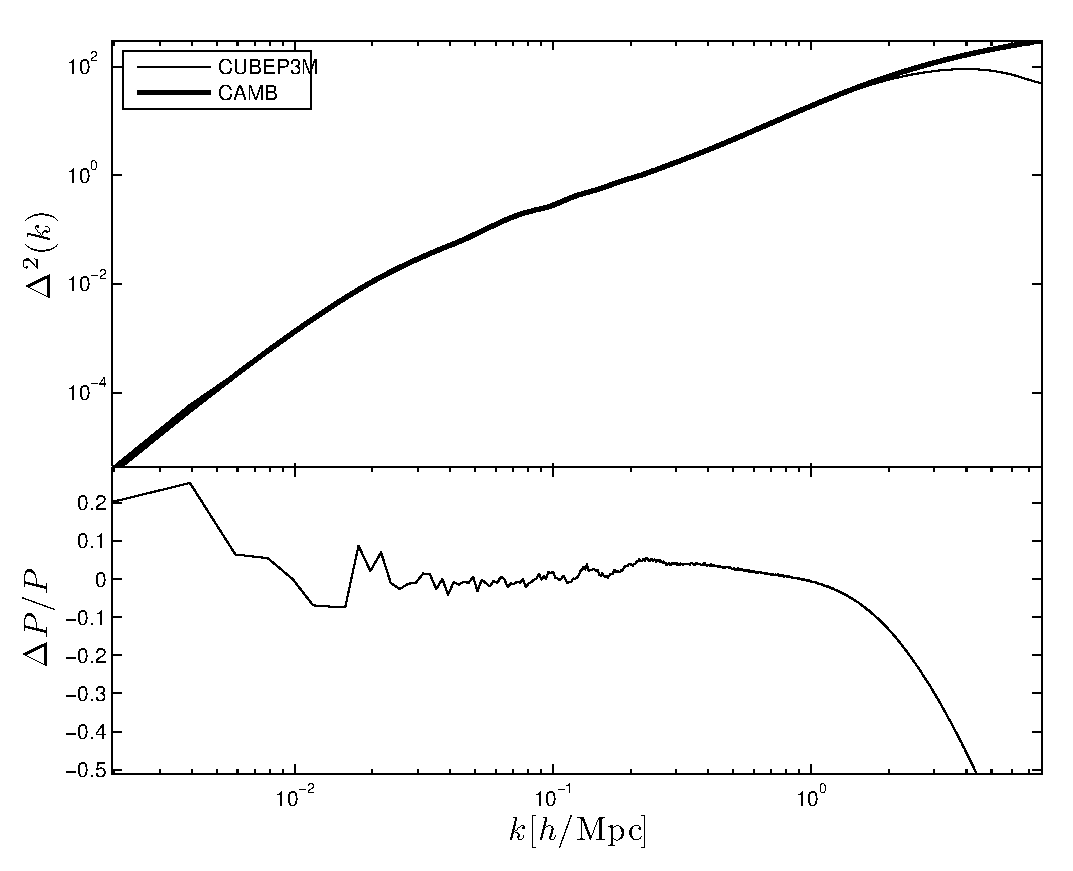
\includegraphics[width=3.2in]{graphs/power_highres.eps}
  \caption{Dark matter power spectrum, measured at $z=0$ in a volume $3.2 h^{-1}\mbox{Gpc}$ per side,
  from $4000^3$ particles. The simulation ran on 4000 cores on RANGER.
    \label{fig:power_highres}}
\end{center}
\end{figure*}

(Show plots of pairwise force (transverse and radial), density force, 
mention the work on covariance matrix by Ngan, Harnoisetal.)


\section{Systematics}
\label{sec:systematics}

To discuss : 

2) choice of initial redshift, which can lead to large truncation error if too early, but poor inaccurate Zel'dovich if too late 
{\bf JD, here you could discuss the ra\_max tempering...} 

3) limits of resolution caused by softening length,

4) Poisson shot noise if too few particles or unrelaxed systems, 

5) finite box size effects (with beat coupling?)
 

The biggest problem with the pp force calculation is that it 
is anisotropic and depends on the location of the fine mesh with respect 
to the particles. An example are two particles on either side of a grid 
cell boundary. These particles will experience the 1-grid cell separation
NGP mesh force, but if the mesh were shifted such that they were
within the same cell, they would experience the (larger) pp force instead. 
This effect is especially pronounced at the early stages of the simulation where
the density is more homogeneous, and leads to mesh artefacts appearing
in the density field. In order to minimize this systematic effect, 
we randomly shift the particle distribution relative to the mesh by a small
amount -- up to 2 fine grid cells in magnitude -- in each
dimension and at each time step.  This adds negligible computational
overhead as it can be applied during the particle position update
and suppresses the mesh behavior over multiple time steps.
It is possible to shift back the particles at the end of each time steps,
which prevents a random drift of the whole population.
This is convenient if one needs to correlate the initial and final positions of the particles.
 
We ensure that, on average, this solution balances out the mesh feature,
by tuning the NGP force kernel such as to provide  force as unbalanced as possible at grid cell distances.
This adjustment is performed from the pairwise force test described in section \ref{sec:accuracy}.
